\documentclass[12pt, twoside]{article}
% \documentclass[12pt, twoside]{article}
\usepackage[letterpaper, margin=1in, headsep=0.2in]{geometry}
\setlength{\headheight}{0.6in}
%\usepackage[english]{babel}
\usepackage[utf8]{inputenc}
\usepackage{microtype}
\usepackage{amsmath}
\usepackage{amssymb}
%\usepackage{amsfonts}
\usepackage[nomessages]{fp} %\FPeval{\var-name}{2*sin(pi/6)}
\usepackage{siunitx} %units in math. eg 20\milli\meter
\usepackage{yhmath} % for arcs, overparenth command
\usepackage{tikz} %graphics
\usetikzlibrary{quotes, angles, arrows, arrows.meta}
\usepackage{graphicx} %consider setting \graphicspath{{images/}}
\usepackage{parskip} %no paragraph indent
\usepackage{enumitem}
\usepackage{multicol}
\usepackage{venndiagram}

\usepackage{fancyhdr}
\pagestyle{fancy}
\fancyhf{}
\renewcommand{\headrulewidth}{0pt} % disable the underline of the header
\raggedbottom
\hfuzz=2mm %suppresses overfull box warnings

\usepackage{hyperref}
\usepackage{float}

\fancyhead[LE]{\thepage}
\fancyhead[RO]{\thepage \\ First and last name: \hspace{2.5cm} \,\\ Section: \hspace{2.5cm} \,}
\fancyhead[LO]{BECA / Dr. Huson / Regents Prep: Graphs\\* 22 October 2024}

\begin{document}

\subsubsection*{1.3 Do Now: Graphing lines and finding intersections}
\begin{enumerate}
  \item Graph and label the two equations. Mark their intersection as an ordered pair.

  \begin{multicols}{2}
    $y = x-5$ \\[0.5cm]
    Write down the slope and $y$-intercept\\ of the first equation.
    \begin{enumerate}
      \item $m=$ \bigskip
      \item $b=$
    \end{enumerate}

    $x+3y = 9$
      \begin{flushleft}
      \begin{tabular}{c|c}
          $x$ & $y$ \\
          \hline
           -3 & 4 \\[5pt]
           0 & 3 \\[5pt]
           3 & 2 \\[5pt]
           6 & 1 \\[5pt]
           9 & 0 \\
          \end{tabular}
        \end{flushleft}
    \end{multicols}

  \begin{center} %4 quadrant regents grid w T-Chart
  \begin{tikzpicture}[scale=.635]
    \draw [help lines] (-10,-10) grid (10,10);
    \draw [thick, ->] (-10.2,0) -- (10.4,0) node [below right] {$x$};
    \draw [thick, ->] (0,-10.2)--(0,10.4) node [left] {$y$};
  \end{tikzpicture}
  \end{center}
Convert the second equation to slope-intercept form, $y=mx+b$.

\newpage
\item In the following problems, solve for the value of $x$, then check your answer.
\begin{multicols}{2}
  \begin{enumerate}[itemsep=5cm]
    \item $2x+3=x + 9$
    \item $\frac{3}{4}x =9$
    \item $3x-3=x + 7$
    \item $\frac{1}{2}(x-7)=12$
    \item $\frac{1}{3} x-7=-4$    
    \item $\frac{2}{3}(x+7)=x-4$
  \end{enumerate}
  \end{multicols} \vspace{4cm}


\item Given the linear function $f(x)=\frac{3}{2}x+4$.
\begin{multicols}{2}
\begin{enumerate}
  \item Find $f(1)$ %\vspace{6cm}
  \item $f(x)=11 \frac{1}{2}$. Find $x$. %\vspace{3cm}
\end{enumerate}
\end{multicols}


\end{enumerate}
\end{document}